\chapter{Opis projektnog zadatka}
		
		%\textbf{\textit{dio 1. revizije}}\\
		
		%\textit{Na osnovi projektnog zadatka detaljno opisati korisničke zahtjeve. Što jasnije opisati cilj projektnog zadatka, razraditi problematiku zadatka, dodati nove aspekte problema i potencijalnih rješenja. Očekuje se minimalno 3, a poželjno 4-5 stranica opisa.	Teme koje treba dodatno razraditi u ovom poglavlju su:}\\
		%\underline{CILJ}\\
		Cilj ovog projektnog zadatka je razviti web aplikaciju „Nestali ljubimci“ koja će korisniku olakšati potragu za odlutalim kućnim ljubimcem. Budući da je informacije o potrazi nepraktično oglašavati putem uobičajenih internetskih platformi za komunikaciju (npr. društvene mreže, stranice za oglašavanje, forumi i slično), ova web aplikacija će vlasnicima životinja, skloništima za životinje i dobrim ljudima koji pomažu u pronalasku životinje omogućiti brz i efikasan način izmjene informacija o nestanku, opažanju i pronalasku odbjeglog kućnog ljubimca. Radi što bržeg pronalaska ljubimca, web aplikacija će biti razvijena za mobilne uređaje kako bi u procesu potrage podržala veću brzinu reagiranja, koja je često ključna za uspješan završetak potrage za kućnim ljubimcem.\\
		
		Prilikom ulaska u web aplikaciju prikazuju se aktivni oglasi, točnije nestali ljubimci. Oglase mogu postaviti uobičajeni korisnici ili skloništa. Poredak oglasa ovisi o načinu pretraživanja koji korisnik odabire. \\
		
		\textbf{KORISNICI}\\
		Aplikacija podržava rad tri tipa korisnika (neregistrirani korisnik, registrirani korisnik i sklonište za životinje).\\
		\underline{Neregistrirani korisnik} pri ulasku u web aplikaciju ima mogućnost pregledavati i pretraživati aktivne oglase o nestalim kućnim ljubimcima. Pretraživanje je ostvareno po kategoriji oglasa i po kategorijama podataka o ljubimcu koje su dostupne pri oglašavanju (vrsta, ime na koje se odaziva, datum i sat nestanka, lokacija nestanka, boja, starost, tekstni opis). Za detaljniji pregled informacija o kućnom ljubimcu kao i za pregled komunikacije o potrazi za njime potrebno je odabrati oglas. Ako neregistrirani korisnik želi sudjelovati u komunikaciji oko potrage za kućnim ljubimcem, potrebna je registracija.
		Podaci potrebni za registraciju su:

		\begin{packed_item}
			\item Ime
			\item Prezime
			\item Korisničko ime
			\item Lozinka
			\item Adresa e-pošte
			\item Broj telefona
	    \end{packed_item}
	    
	    
	   	\begin{figure}[H]
	   		
	   		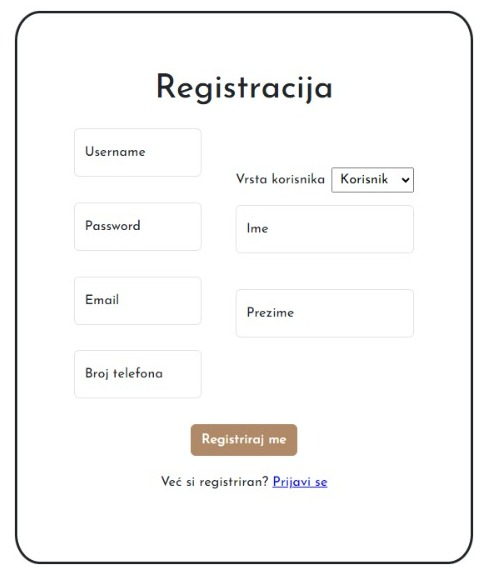
\includegraphics[scale =0.4]{registracija.JPEG}
	   		\centering
	   		\caption{Registracija}
	   		\label{fig:your_label}
	   \end{figure}
	   
	   \begin{figure}[H]
	   	
	   	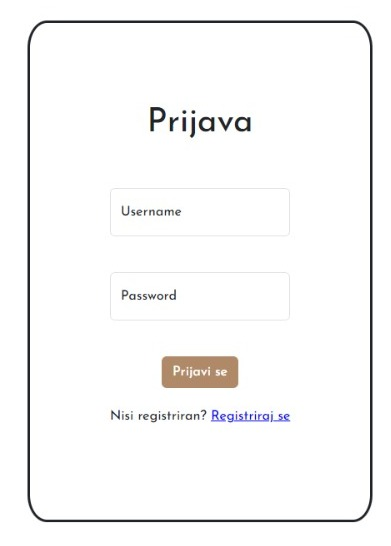
\includegraphics[scale =0.4]{prijava.JPEG}
	   	\centering
	   	\caption{Prijava}
	   	\label{fig:your_label}
	   \end{figure}
	   
	   
	     
	    
	    \underline{Registrirani korisnik}, koji osim svih mogućnosti koje ima i neregistrirani korisnik, dodatno ima sljedeće mogućnosti:
	     
		\begin{packed_item}
			\item Postavljanje oglasa o nestalom kućnom ljubimcu 
			\item Sudjelovanje u komunikaciji oko potrage za ljubimcem
			\item Uklanjanje oglasa o nestalom kućnom ljubimcu
			\item Izmjena oglasa o nestalom kućnom ljubimcu
		\end{packed_item}
		Treći tip korisnika su \underline{skloništa za životinje}, koji osim svih mogućnosti koje ima registrirani korisnik, ima dodatnu mogućnost oglašavanja životinja koje su pronađene i nalaze se u njihovom prostoru. Skloništa za životinje pri registraciji moraju unijeti i naziv skloništa.\\
		
		
		\textbf{OGLASI}\\
		Za \underline{postavljanje oglasa} potrebno je unijeti sljedeće informacije o ljubimcu:
		\begin{packed_item}
			\item Vrsta
			\item Ime na koje se odaziva
			\item Datum i sat nestanka
			\item Lokacija nestanka
			\item Boja
			\item Starost
			\item Tekstni opis
			\item Slike (najviše 3 slike)
		\end{packed_item}
		Pri pretraživanju kućnih ljubimaca, vrsta je podijeljena u kategorije: pas, mačka, ptica, glodavac, kunić, gmaz te ostalo.\\
		Uz to, postoje kategorije za boju (crna, smeđa, bijela, siva, zelena, crvena, crna, žuta, narančasta, plava, šarena) i za starost. Starost je podijeljena u intervale: $<$1god., 1god., 2god., 3god., 4-5god., 6-10god. i $>$10god.
		Osim podataka o kućnom ljubimcu, oglas sadrži i kontakt podatke korisnika koji se povlače iz korisničkih podataka danih pri registraciji (adresa e-pošte, broj telefona).\\
		Oglas mora imati jednu od \underline{kategorija}:
		\begin{packed_item}
			\item Za ljubimcem se traga
			\item Ljubimac je sretno pronađen
			\item Ljubimac nije pronađen, ali se za njim više ne traga aktivno
			\item Ljubimac je pronađen uz nesretne okolnosti
			\item U skloništu 
		\end{packed_item}
		\begin{figure}[H]
			
			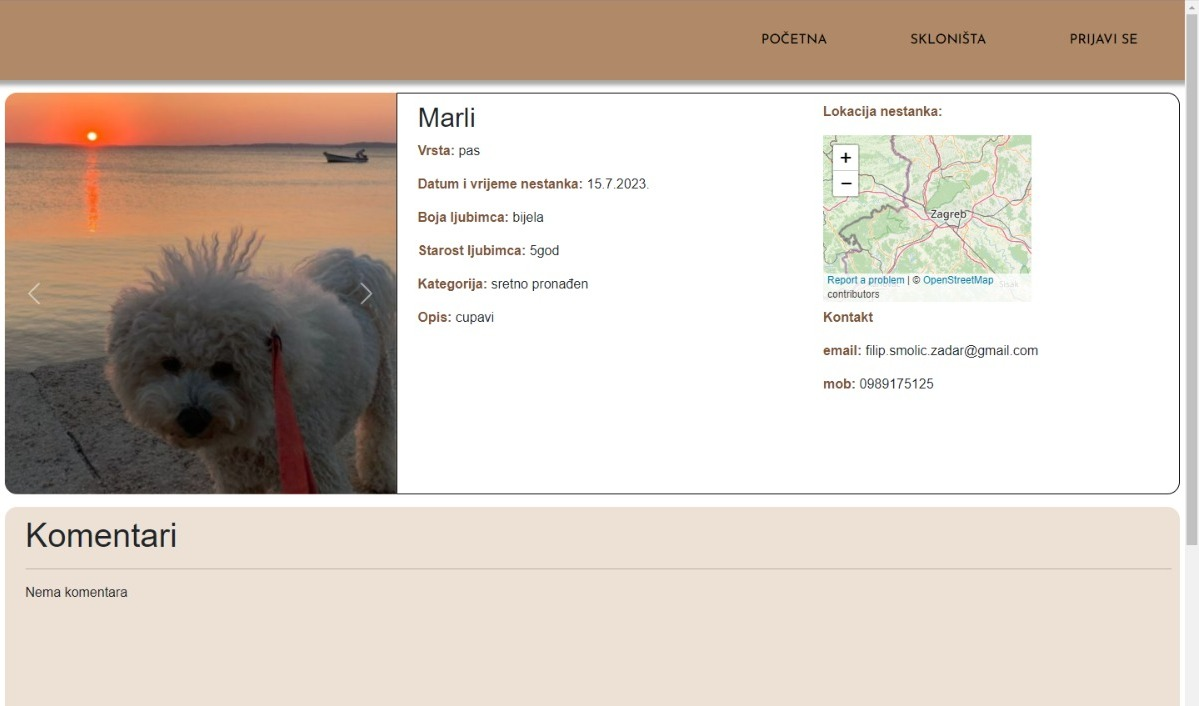
\includegraphics[scale =0.4]{oglas.JPEG}
			\centering
			\caption{Primjer oglasa}
			\label{fig:your_label}
		\end{figure}
		
		Od ovih kategorija inicijalno je postavljena da se za ljubimcem traga. Kategoriju 'U skloništu' imaju mogućnost postaviti samo prijavljena skloništa za životinje. Na oglasu je moguća
		 \underline{izmjena} svih kategorija podataka o ljubimcima, kao i kategorija oglasa. Sve kategorije, osim da se za ljubimcem aktivno traga, oglas čine neaktivnim. Također, web aplikacija sadrži popis neaktivnih oglasa koje mogu pregledavati samo registrirani korisnici.\\
		\underline{Komunikacija} oko potrage za kućnim ljubimcem odvijat će se porukama koje mogu sadržavati:
		\begin{packed_item}
			\item Tekst
			\item Sliku
			\item Geolokaciju
		\end{packed_item}
		uz kontakt podatke o osobi koja komunicira. Geolokacija je izvedena uz pomoć vanjske usluge OpenStreetMap.\\
		
		\textbf{Ostalo}\\
		Aplikacija je izvedena kao mobilna aplikacija.\\
		Sustav podržava rad više korisnika u stvarnom vremenu. Također, sustav podržava hrvatski jezik.\\
		Aplikacija je namijenjena vlasnicima izgubljenih ljubimaca i svim dobrim dušama koje su voljne pomoći oko potrage za nestalim kućnim ljubimcima.\\
		
		\textbf{Moguća buduća proširenja aplikacije:}
		\begin{packed_item}
			\item obavještavanje vlasnika izgubljenog kućnog ljubimca nakon što korisnik ostavi komentar na njegovom oglasu
			\item integracija s postojećim društvenim mrežama
		\end{packed_item}
		
		%\begin{packed_item}
			%\item \textit{potencijalna korist ovog projekta}
			%\item \textit{postojeća slična rješenja (istražiti i ukratko opisati razlike u odnosu na zadani zadatak). Dodajte slike koja predočavaju slična rješenja.}
			%\item \textit{skup korisnika koji bi mogao biti zainteresiran za ostvareno rješenje.}
			%\item \textit{mogućnost prilagodbe rješenja }
			%\item \textit{opseg projektnog zadatka}
			%\item \textit{moguće nadogradnje projektnog zadatka}
		%\end{packed_item}
		
		%\textit{Za pomoć pogledati reference navedene u poglavlju „Popis literature“, a po potrebi konzultirati sadržaj na internetu koji nudi dobre smjernice u tom pogledu.}
		\eject
		
		%\section{Primjeri u \LaTeX u}
		
		%\textit{Ovo potpoglavlje izbrisati.}\\

		%U nastavku se nalaze različiti primjeri kako koristiti osnovne funkcionalnosti \LaTeX a koje su potrebne za izradu dokumentacije. Za dodatnu pomoć obratiti se asistentu na projektu ili potražiti upute na sljedećim web sjedištima:
		%\begin{itemize}
			%\item Upute za izradu diplomskog rada u \LaTeX u - \url{https://www.fer.unizg.hr/_download/repository/LaTeX-upute.pdf}
			%\item \LaTeX\ projekt - \url{https://www.latex-project.org/help/}
			%\item StackExchange za Tex - \url{https://tex.stackexchange.com/}\\
		
		%\end{itemize} 	


		
		%\noindent \underbar{podcrtani tekst}, \textbf{podebljani tekst}, 	\textit{nagnuti tekst}\\
		%\noindent \normalsize primjer \large primjer \Large primjer \LARGE {primjer} \huge {primjer} \Huge primjer %\normalsize
				
		%\begin{packed_item}
			
			%\item  primjer
			%\item  primjer
			%\item  primjer
			%\item[] \begin{packed_enum}
				%\item primjer
				%\item[] \begin{packed_enum}
					%\item[1.a] primjer
					%\item[b] primjer
				%\end{packed_enum}
				%\item primjer
			%\end{packed_enum}
			
		%\end{packed_item}
		
		%\noindent primjer url-a: \url{https://www.fer.unizg.hr/predmet/proinz/projekt}
		
		%\noindent posebni znakovi: \# \$ \% \& \{ \} \_ 
		%$|$ $<$ $>$ 
		%\^{} 
		%\~{} 
		%$\backslash$ 
		
		
		%\begin{longtblr}[
			%label=none,
			%entry=none
			%]{
			%	width = \textwidth,
			%	colspec={|X[8,l]|X[8, l]|X[16, l]|}, 
			%	rowhead = 1,
			%} %definicija širine tablice, širine stupaca, poravnanje i broja redaka naslova tablice
			%\hline \SetCell[c=3]{c}{\textbf{naslov unutar tablice}}	 \\ \hline[3pt]
			%\SetCell{LightGreen}IDKorisnik & INT	&  	Lorem ipsum dolor sit amet, consectetur adipiscing elit, sed do eiusmod  	\\ \hline
			%korisnickoIme	& VARCHAR &   	\\ \hline 
			%email & VARCHAR &   \\ \hline 
			%ime & VARCHAR	&  		\\ \hline 
			%\SetCell{LightBlue} primjer	& VARCHAR &   	\\ \hline 
		%\end{longtblr}
		

		%\begin{longtblr}[
				%caption = {Naslov s referencom izvan tablice},
				%entry = {Short Caption},
			%]{
				%width = \textwidth, 
				%colspec = {|X[8,l]|X[8,l]|X[16,l]|}, 
				%rowhead = 1,
			%}
			%\hline
			%\SetCell{LightGreen}IDKorisnik & INT	&  	Lorem ipsum dolor sit amet, consectetur adipiscing elit, sed do eiusmod  	\\ \hline
			%korisnickoIme	& VARCHAR &   	\\ \hline 
			%email & VARCHAR &   \\ \hline 
			%ime & VARCHAR	&  		\\ \hline 
			%\SetCell{LightBlue} primjer	& VARCHAR &   	\\ \hline 
		%\end{longtblr}
	


		
		
		%unos slike
		%\begin{figure}[H]
			%\includegraphics[scale=0.4]{slike/aktivnost.PNG} %veličina slike u odnosu na originalnu datoteku i pozicija slike
			%\centering
			%\caption{Primjer slike s potpisom}
			%\label{fig:promjene}
		%\end{figure}
		
		%\begin{figure}[H]
			%\includegraphics[width=\textwidth]{slike/aktivnost.PNG} %veličina u odnosu na širinu linije
			%\caption{Primjer slike s potpisom 2}
			%\label{fig:promjene2} %label mora biti drugaciji za svaku sliku
		%\end{figure}
		
		%Referenciranje slike \ref{fig:promjene2} u tekstu.
		
		%\eject
		
	